\documentclass[a4paper, 12pt]{article}
\usepackage[T2A,T1]{fontenc}
\usepackage[utf8]{inputenc}
\usepackage[english, russian]{babel}
\usepackage{graphicx}
\usepackage[hcentering, bindingoffset = 10mm, right = 15 mm, left = 15 mm, top=20mm, bottom = 20 mm]{geometry}
\usepackage{multirow}
\usepackage{lipsum}
\usepackage{amsmath, amstext}
\usepackage{siunitx}
\usepackage{subcaption}
\usepackage{wrapfig}
\usepackage{adjustbox}
\usepackage{enumerate, indentfirst, float}
\usepackage{capt-of, svg}
\usepackage{icomma}

\newenvironment{bottompar}{\par\vspace*{\fill}}{\clearpage}
 
\begin{document}
\begin{titlepage}

\newcommand{\HRule}{\rule{\linewidth}{0.5mm}} % Defines a new command for the horizontal lines, change thickness here

\center % Center everything on the page
 
%----------------------------------------------------------------------------------------
%	HEADING SECTIONS
%----------------------------------------------------------------------------------------

\textsc{\LARGE Московский \\[0.5cm]Физико-Технический Институт}\\[1,5cm] % Name of your university/college
\textsc{\Large Кафедра общей физики}\\[0.5cm] % Major heading such as course name
\textsc{\large Лабораторная работа \textnumero  3.2.1}\\[0.5cm] % Minor heading such as course title

%----------------------------------------------------------------------------------------
%	TITLE SECTION
%----------------------------------------------------------------------------------------

\HRule
\\[0.4cm]
{ \huge \bfseries Сдвиг фаз в цепи переменного тока}
\\[0.2cm] % Title of your document
\HRule
\\[1.5cm]


 
%----------------------------------------------------------------------------------------
%	AUTHOR SECTION
%----------------------------------------------------------------------------------------


	\begin{flushleft} \large
		\emph{Студент:}\\
		Павел \textsc{Северилов} \\
		671 группа
	\end{flushleft}



\begin{bottompar}
	\begin{center}
		
\includegraphics[width = 80 mm]{logo.jpg}
	\end{center}
	{\large \today}

\end{bottompar}
\vfill

\end{titlepage}

\section{Цель работы}
Изучить влияние активного сопротивления, индуктивности и емкости на сдвиг фаз между током и напряжением в цепи переменного тока.

\subsection*{Экспериментальная установка}



\begin {figure}[H]
\begin{center}
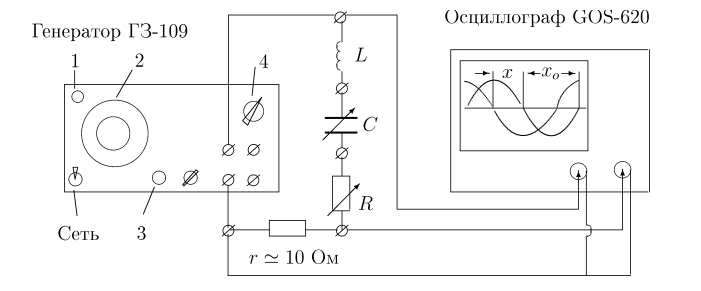
\includegraphics[width=0.9\textwidth]{t}
\end{center}
\end {figure}


\subsection*{RC-цепь}


Ток, текущий через RC цепочку, пропорционален напряжению на резисторе, и опережает напряжение на конденсаторе по фазе на $\pi/2$. В данном случае получаем теоретический результат для зависимости сдвига фаз от $R$:
$$\tg \varphi = \frac{1}{\Omega R C}$$

\subsection*{RL-цепь}

Всё аналогично RC цепочке, только импеданс катушки теперь 
$$Z_2 = j\omega L,$$
поэтому ток отстаёт по фазе от напряжения, а рассчётная формула приобретает вид
$$\tg \varphi = \frac{\omega L}{R_{\sum}}$$
Теперь к споротивлению калибровочного резистора и резистора $R$ добавится активное сопротивление катушки:
$$R_{\sum} = R+r+R_L,$$
где $R_L$ -- активное сопротивление катушки.

\subsection*{RCL-цепь}

Комплексный импеданс RCL-цепочки:
$$Z=R+j\omega L - \frac{j}{\omega C}.$$

Сдвиг фаз между током и напряжением получим, взяв аргумент $Z$:

$$\tg\varphi = \frac{\omega L - \frac{1}{\omega C}}{R} = Q\frac{\left(\frac{\omega}{\omega_0}\right)^2 - 1}{\frac{\omega}{\omega_0}} = Q\frac{(1+x)^2-1}{1+x} \simeq 2x Q,$$
где $x = \Delta \omega / \omega_0 = \Delta \nu / \nu_0$, и в последнем переходе пренебрегаем квадратичными по $x$ членами.
Измерив ширину графика $w=2x$ на высоте $\varphi = \pi / 4\ (\tg\varphi = 1)$, можем непосредственно измерить добротность контура:
$$Q = \frac{1}{w}$$

\subsection*{Фазовращатель}

\begin {figure}[H]
\begin{center}
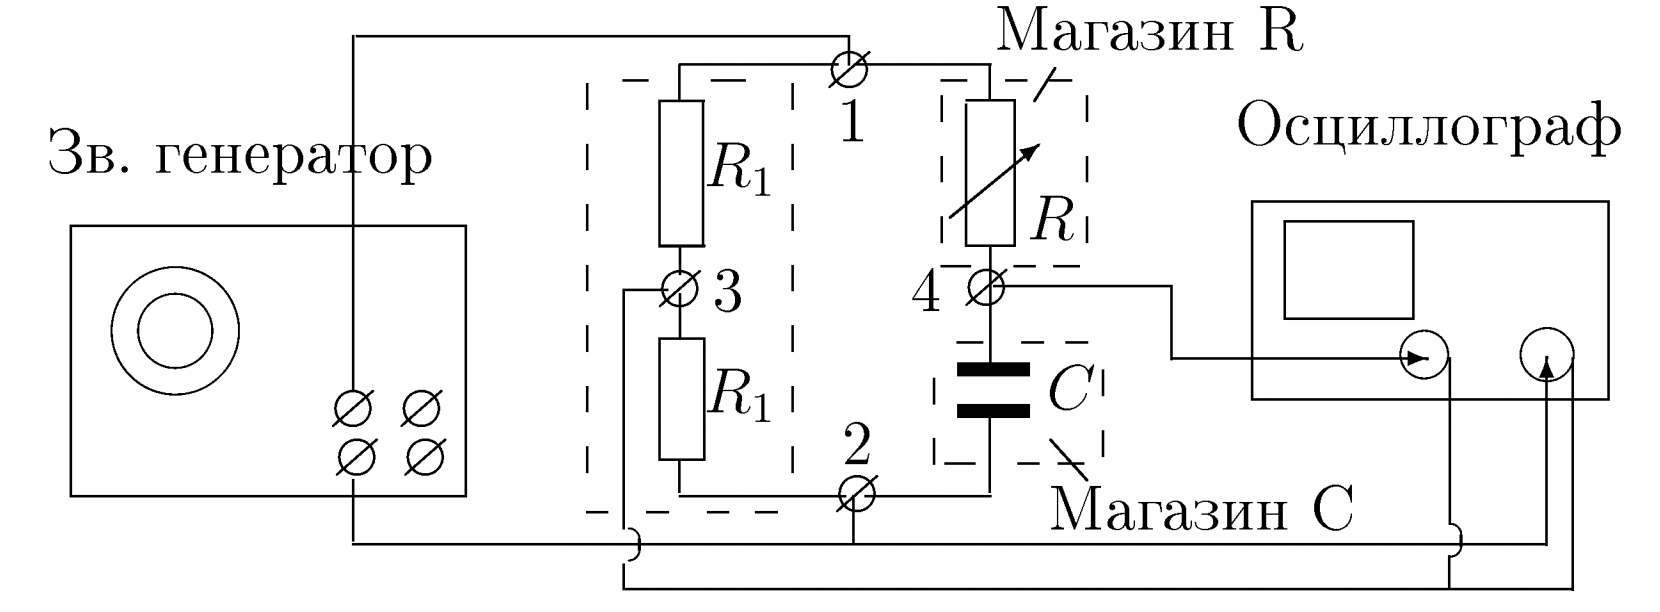
\includegraphics[width=0.8\textwidth]{phase.png}
\end{center}
\end {figure}

Построим векторную диаграмму для фазовращателя:
\begin {figure}[H]
\begin{center}
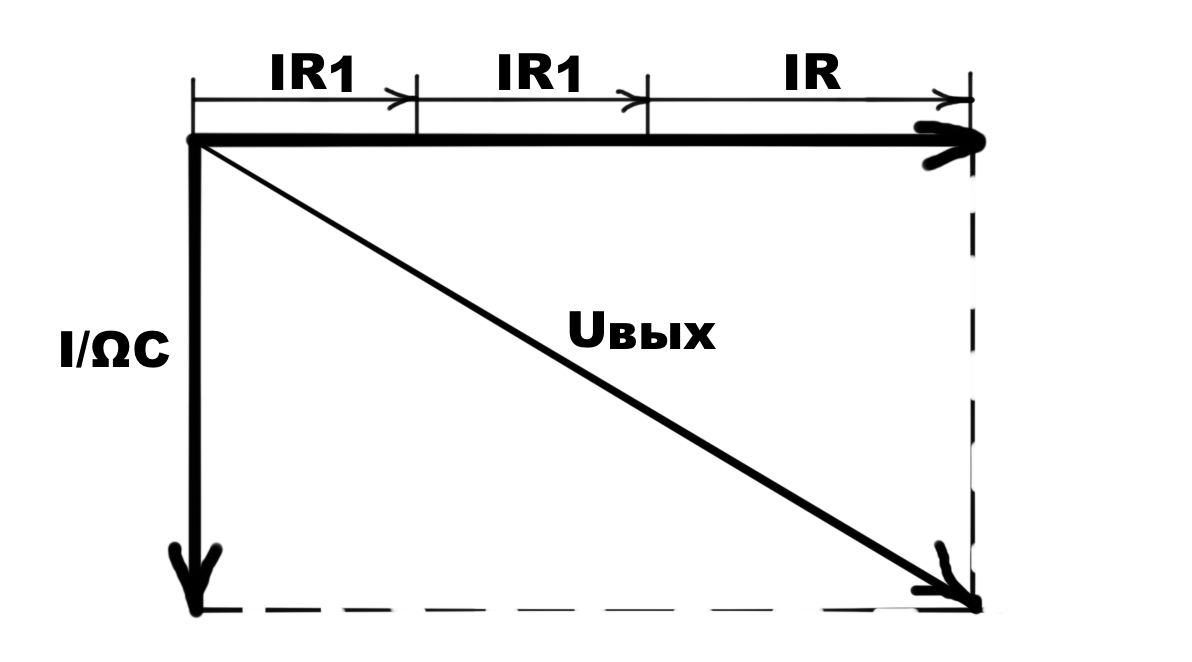
\includegraphics[width=0.7\textwidth]{diagram}
\end{center}
\end {figure}



\newpage
\section{Работа и измерения}

Везде будем считать, что $\sigma_x=0.1$. Запишем показания приборов: 
$$C = 0.5 \text{ мкФ},
L =50 \text{ мГн},
\nu = 1 \text{ кГц},
R_L = 31.5 \text{ Ом},
r = 12,4 \text{ Ом}$$

\subsection*{RC-цепь}
Измерим сдвиг фаз в RC-цепи в зависимости от сопротивления. Результаты занесем в таблицу 1.
$$X_1 = \dfrac{1}{2 \pi \nu C} = 318.2\text{ Ом};~~R_{\Sigma} =R+r $$

\begin{table}[H]
\centering
\begin{tabular}{|c|c|c|c|c|c|c|c|}
\hline
$R, \text{ Ом}$ & $x$ & $x_0$ & $\psi$ & $\tg \psi$ & $R_{\Sigma}, \text{ Ом}$ & $1/(R_{\Sigma} \Omega C)$ & $\sigma_{tg\psi}$\\ \hline
0&	1,2&	2,5&	1,51&	15,89&	12,4&	25,661&	0,14\\ \hline
100&	1,1&	2,4&	1,44&	7,60&	112,4&	2,831&	0,14\\ \hline
200&	0,8&	2,4&	1,05&	1,73&	212,4&	1,498&	0,14\\ \hline
300&	0,65&	2,4&	0,85&	1,14&	312,4&	1,019&	0,14\\ \hline
400&	0,55&	2,4&	0,72&	0,88&	412,4&	0,772&	0,14\\ \hline
500&	0,45&	2,4&	0,59&	0,67&	512,4&	0,621&	0,13\\ \hline
700&	0,35&	2,4&	0,46&	0,49&	712,4&	0,447&	0,13\\ \hline
900&	0,3&	2,4&	0,39&	0,41&	912,4&	0,349&	0,13\\ \hline
1100&	0,25&	2,4&	0,33&	0,34&	1112,4&	0,286&	0,13\\ \hline
\end{tabular}
\caption{Полученные значения в RC-цепи}
\end{table}

	\begin {figure}[H]
		\begin{center}
			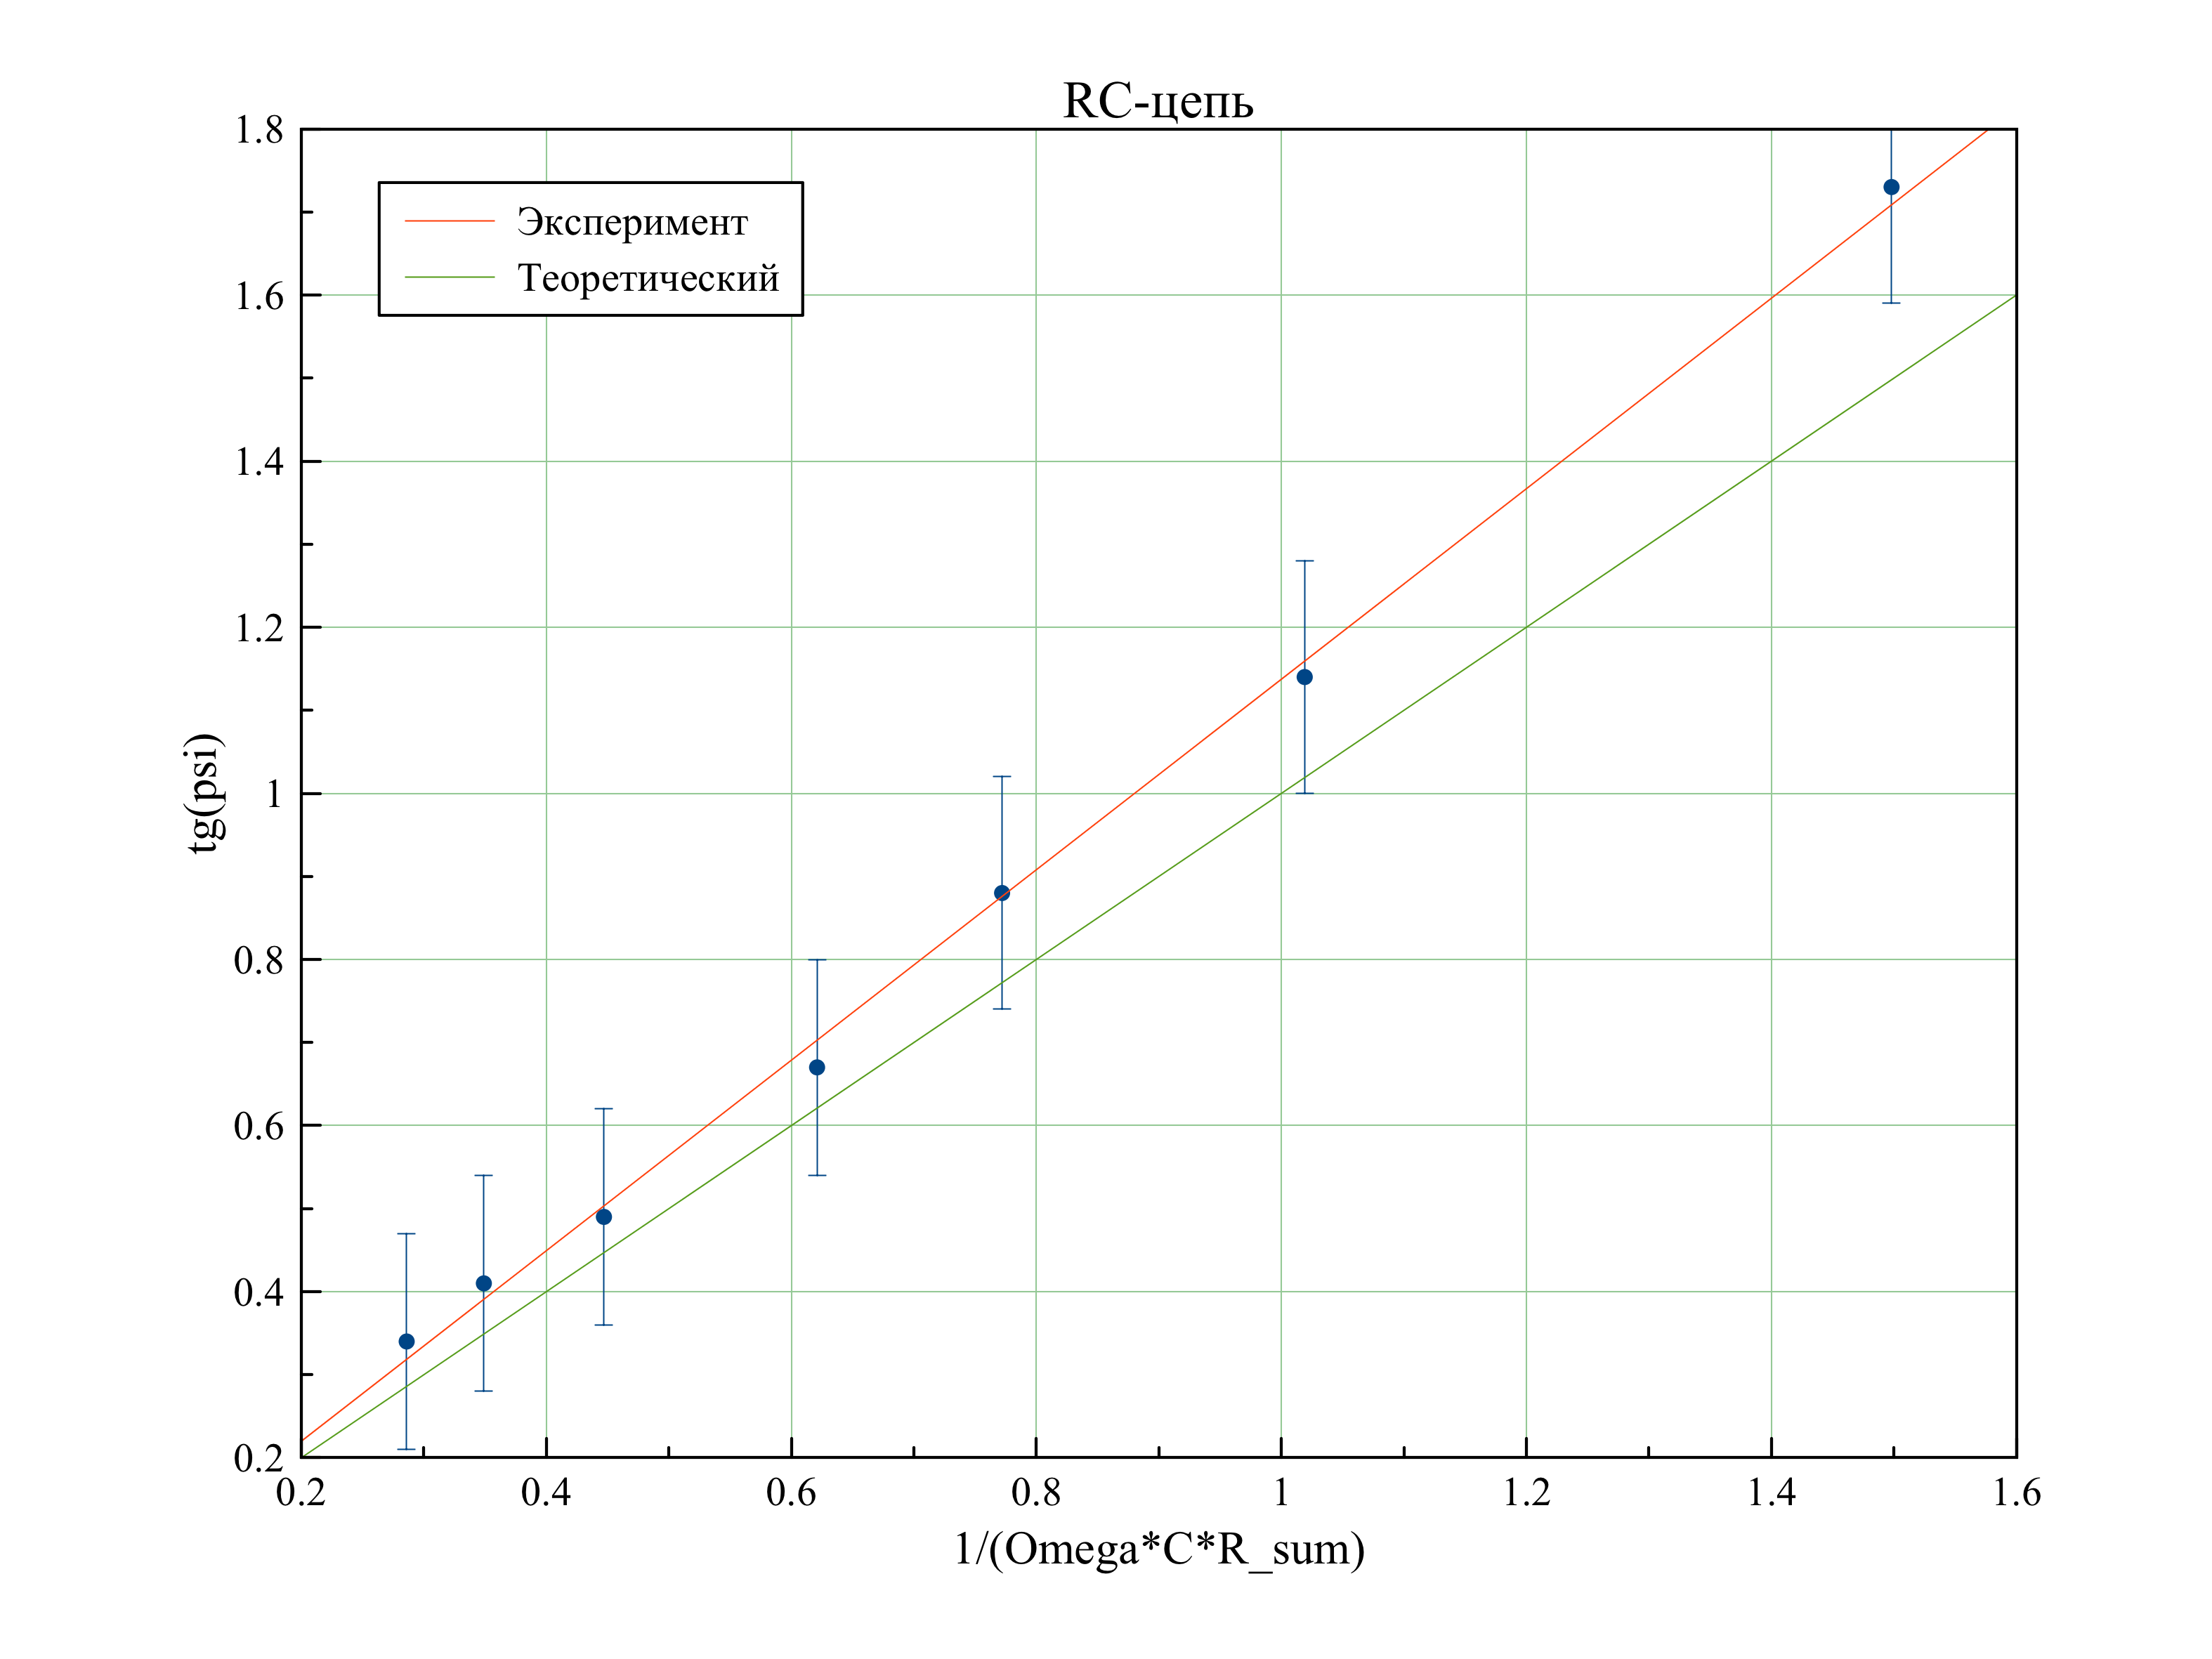
\includegraphics[width=0.9\textwidth]{RC}
			\caption{График зависимости $\tg \psi = f[1/ \Omega C R_{\Sigma}]$}
		\end{center}
	\end {figure}

\subsection*{RL-цепь}
Проделаем аналогичные измерения для RL-цепи
$$X_2 = 2 \pi \nu L = 314.16$$

\begin{table}[H]
\centering
\begin{tabular}{|c|c|c|c|c|c|c|c|}
\hline
$R, \text{ Ом}$ & $x$ & $x_0$ & $\psi$ & $\tg \psi$ & $R_{\Sigma}$ & $\Omega L/ R_{\Sigma} $ & $\sigma_{\tg\psi}$ \\ \hline
0&	1,1&	2,4&	1,440&	7,596&	43,9& 7,16&	0,145\\ \hline
100&	0,85&	2,4&	1,113&	2,028&	143,9& 2,18&	0,140\\ \hline
200&	0,7&	2,4&	0,916&	1,303&	243,9& 1,29&	0,137\\ \hline
400&	0,5&	2,4&	0,654&	0,767&	443,9& 0,71&	0,135\\ \hline
600&	0,35&	2,4&	0,458&	0,493&	643,9& 0,49&	0,133\\ \hline
800&	0,3&	2,4&	0,393&	0,414&	843,9& 0,37&	0,133\\ \hline
1000&	0,25&	2,4&	0,327&	0,339&	1043,9& 0,30&	0,132\\ \hline
\end{tabular}
\caption{Полученные значения в RL-цепи}
\end{table}

\begin {figure}[H]
	\begin{center}
		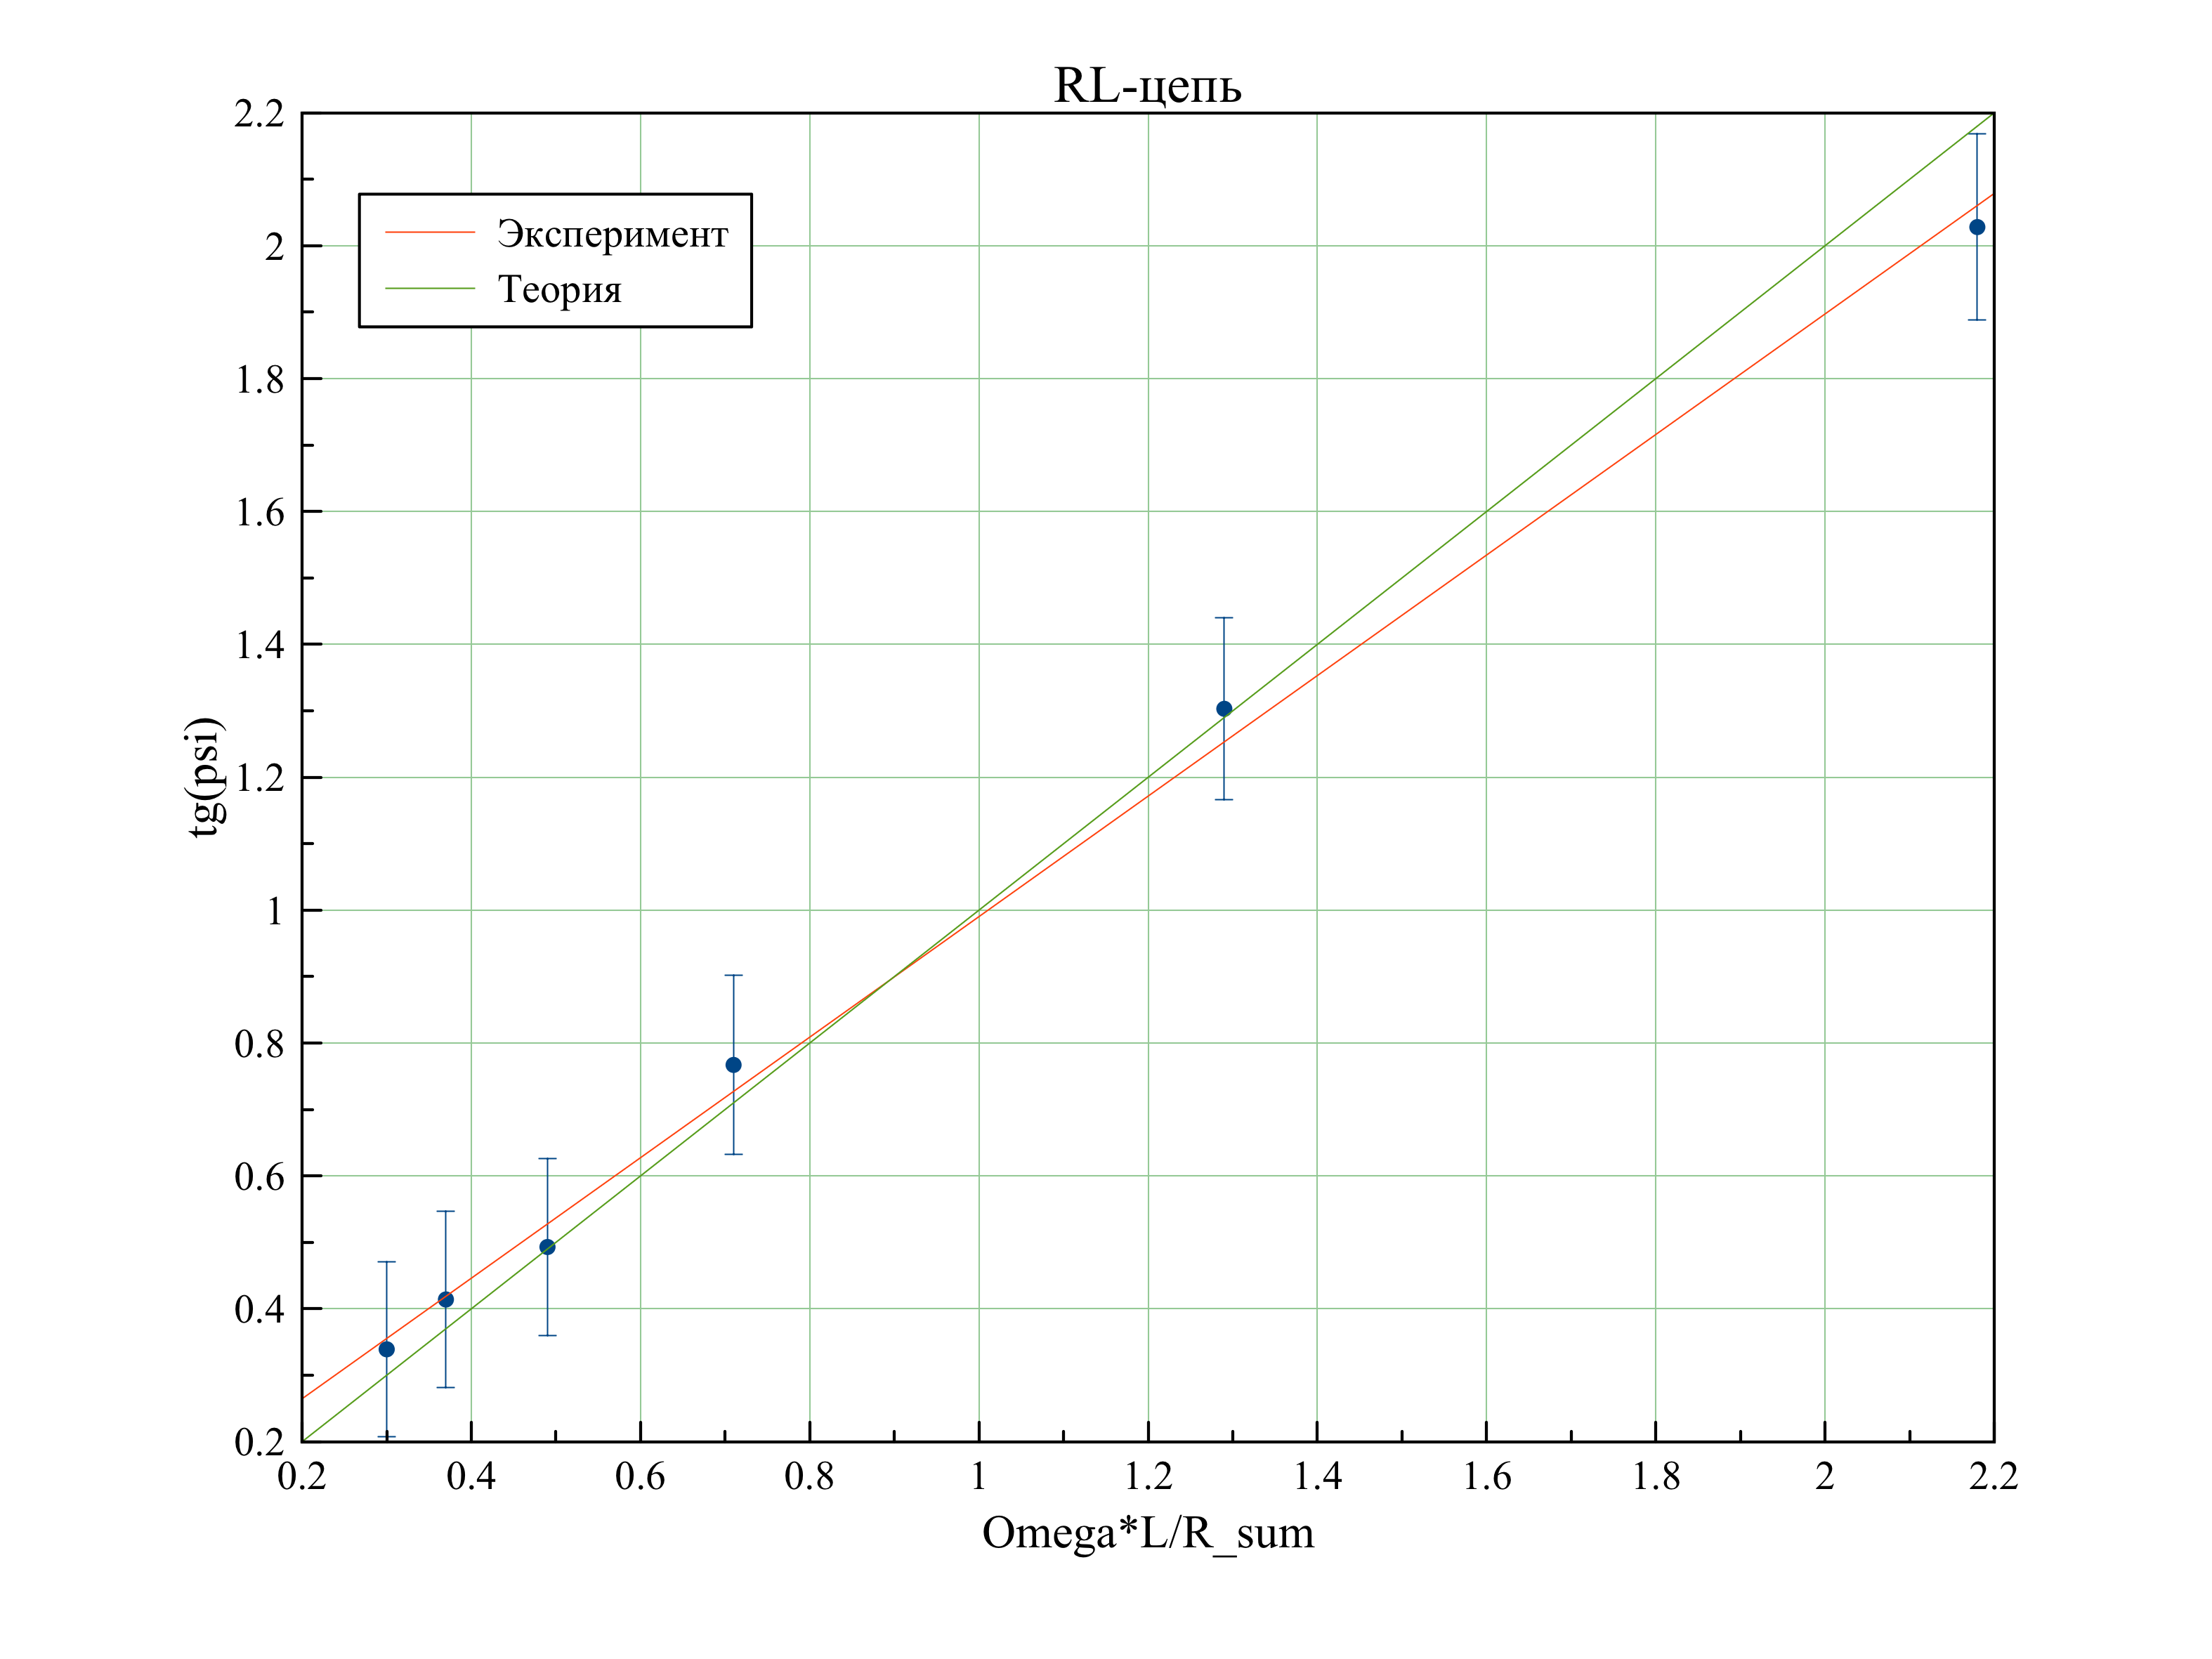
\includegraphics[width=0.9\textwidth]{RL}
		\caption{График зависимости $\tg \psi = f[\Omega L / R_{\Sigma}]$}
	\end{center}
\end {figure}

\subsection*{RCL-цепь}
Расчитаем резонансную частоту $\nu_0 = \cfrac{1}{2\pi\sqrt{LC}} = 1006.6 \text{ Гц}$. 

Меняя частоту в обе стороны от резонансного значения, полученного подбором на установке, снимем зависимость сдвига фаз от частоты. Проделаем измерения для двух сопротивлений: $R=0\text{ Ом}; R=100\text{ Ом}$. Результаты заносим в таблицу.
\begin{table}[H]
\centering
\begin{tabular}{|c|c|c|c|c|c|c|c|}
\hline
Сопротивление & $\nu, \text{Гц}$ & $x$ & $x_0$ & $\nu/\nu_0$ & $|\psi|$ &$\sigma_{\nu/\nu_0}$& $\sigma_{\psi}$\\ \hline
\multirow{11}{*}{$R = 0 \; \text{Ом}$}   
										 &1020	&0		&4,9	&1,013	&0,000	&0,010	&0,000 \\ \cline{2-8}
										 &1000	&0,4	&4,9	&0,993	&0,256	&0,010	&0,064 \\ \cline{2-8} 
										 &980	&0,9	&5,2	&0,974	&0,544	&0,010	&0,061 \\ \cline{2-8} 
										 &960	&1,2	&5,2	&0,954	&0,725	&0,010	&0,062 \\ \cline{2-8} 
										 &940	&1,5	&5,3	&0,934	&0,889	&0,011	&0,062 \\ \cline{2-8} 
										 &930	&1,7	&5,4	&0,924	&0,989	&0,011	&0,061 \\ \cline{2-8}
										 &1040	&0,8	&4,9	&1,033	&0,513	&0,010	&0,065 \\ \cline{2-8} 
										 &1060	&1,1	&4,9	&1,053	&0,705	&0,009	&0,066 \\ \cline{2-8} 
										 &1080	&1,3	&4,7	&1,073	&0,869	&0,009	&0,069 \\ \cline{2-8} 
										 &1100	&1,5	&4,8	&1,093	&0,982	&0,009	&0,069 \\ \cline{2-8} 
										 &1120	&1,6	&4,5	&1,113	&1,117	&0,009	&0,074 \\ \hline 
\multirow{13}{*}{$R = 100 \; \text{Ом}$} 
										&1020	&0		&4,8	&1,013	&0,000	&0,010	&0,000\\ \cline{2-8}
										&1000	&0,1	&5,0	&0,993	&0,063	&0,010	&0,063\\ \cline{2-8}
										&980	&0,2	&5,2	&0,974	&0,121	&0,010	&0,060\\ \cline{2-8}
										&960	&0,4	&5,3	&0,954	&0,237	&0,010	&0,059\\ \cline{2-8}
										&940	&0,5	&5,3	&0,934	&0,296	&0,010	&0,060\\ \cline{2-8}
										&930	&0,6	&5,4	&0,924	&0,349	&0,010	&0,059\\ \cline{2-8}
										&1040	&0,2	&4,9	&1,033	&0,128	&0,010	&0,064\\ \cline{2-8}
										&1060	&0,3	&4,7	&1,053	&0,201	&0,010	&0,067\\ \cline{2-8}
										&1080	&0,4	&4,6	&1,073	&0,273	&0,010	&0,069\\ \cline{2-8}
										&1100	&0,5	&4,6	&1,093	&0,341	&0,010	&0,069\\ \cline{2-8}
										&1120	&0,6	&4,5	&1,113	&0,419	&0,010	&0,070 \\ \hline 
\end{tabular}
\caption{Полученные значения при изучении зависимости фазы от $\dfrac{\nu}{\nu_0}$}
\end{table}


\begin {figure}[H]
	\begin{center}
		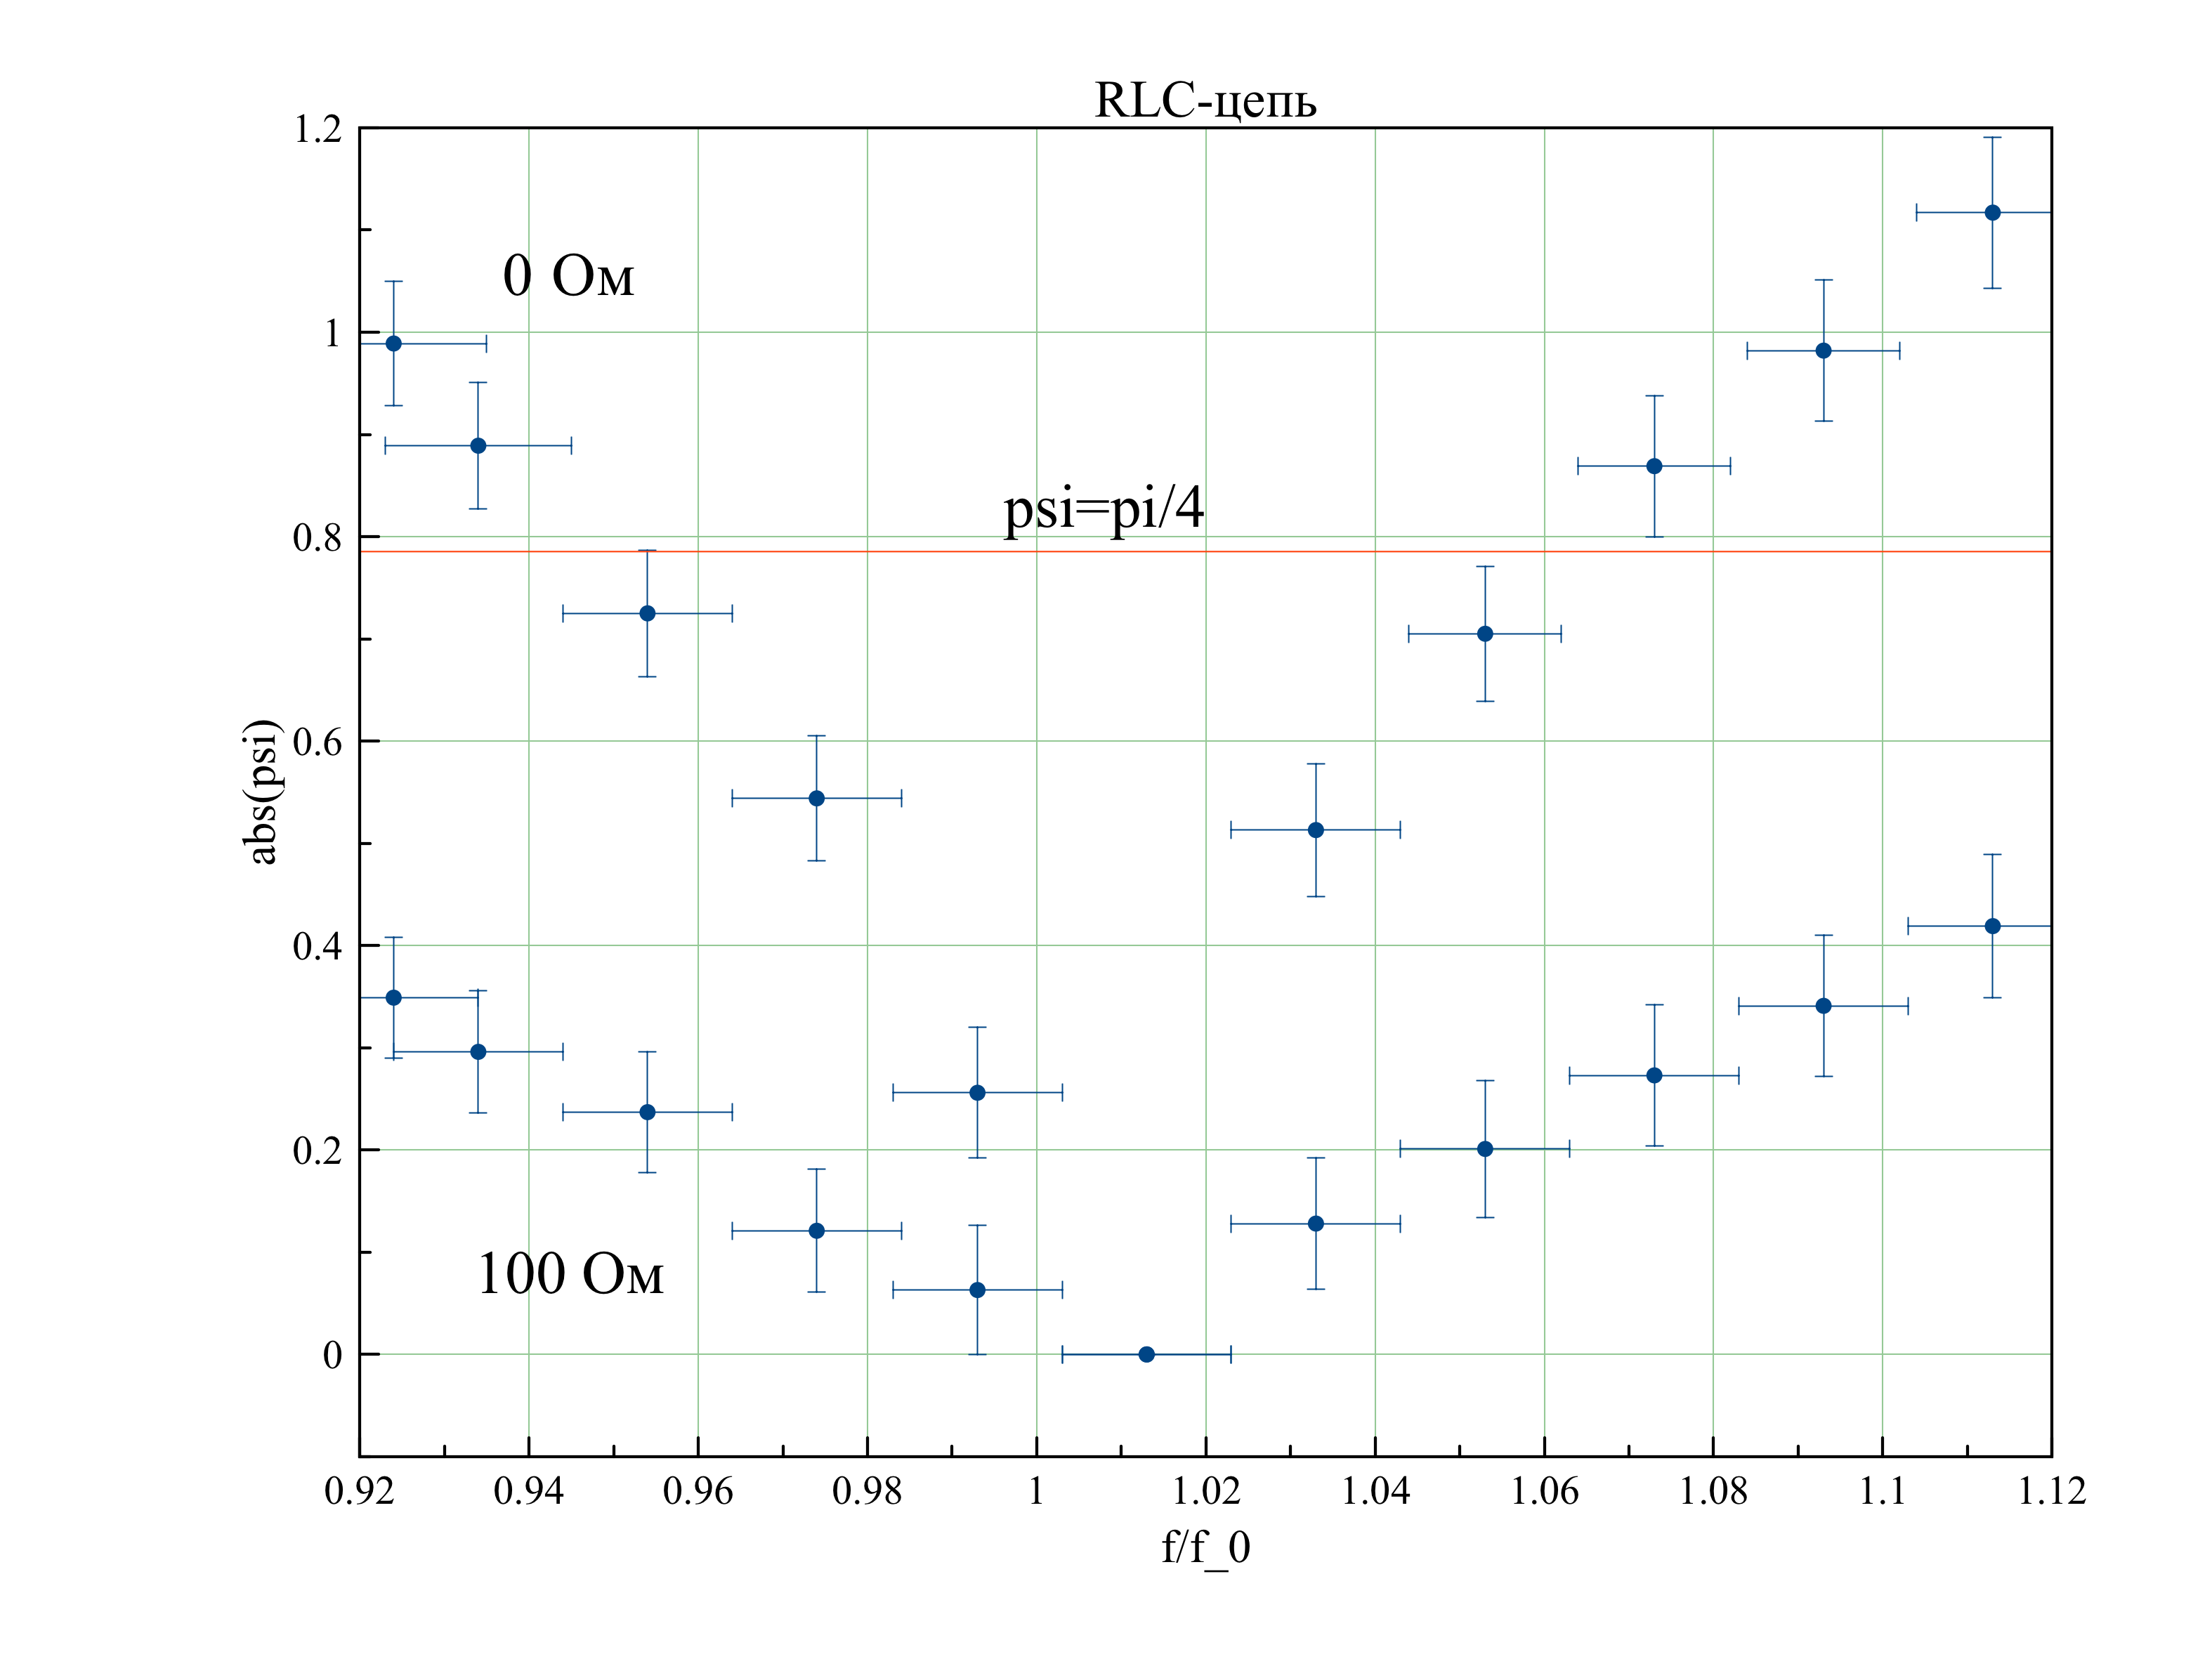
\includegraphics[width=0.8\textwidth]{RLC}
		\caption{График зависимости $\psi = f[\nu/\nu_0] \text{ для $R = 0$ Ом и $R = 100$ Ом}$}
	\end{center}
\end {figure}

\begin {figure}[H]
	\begin{center}
		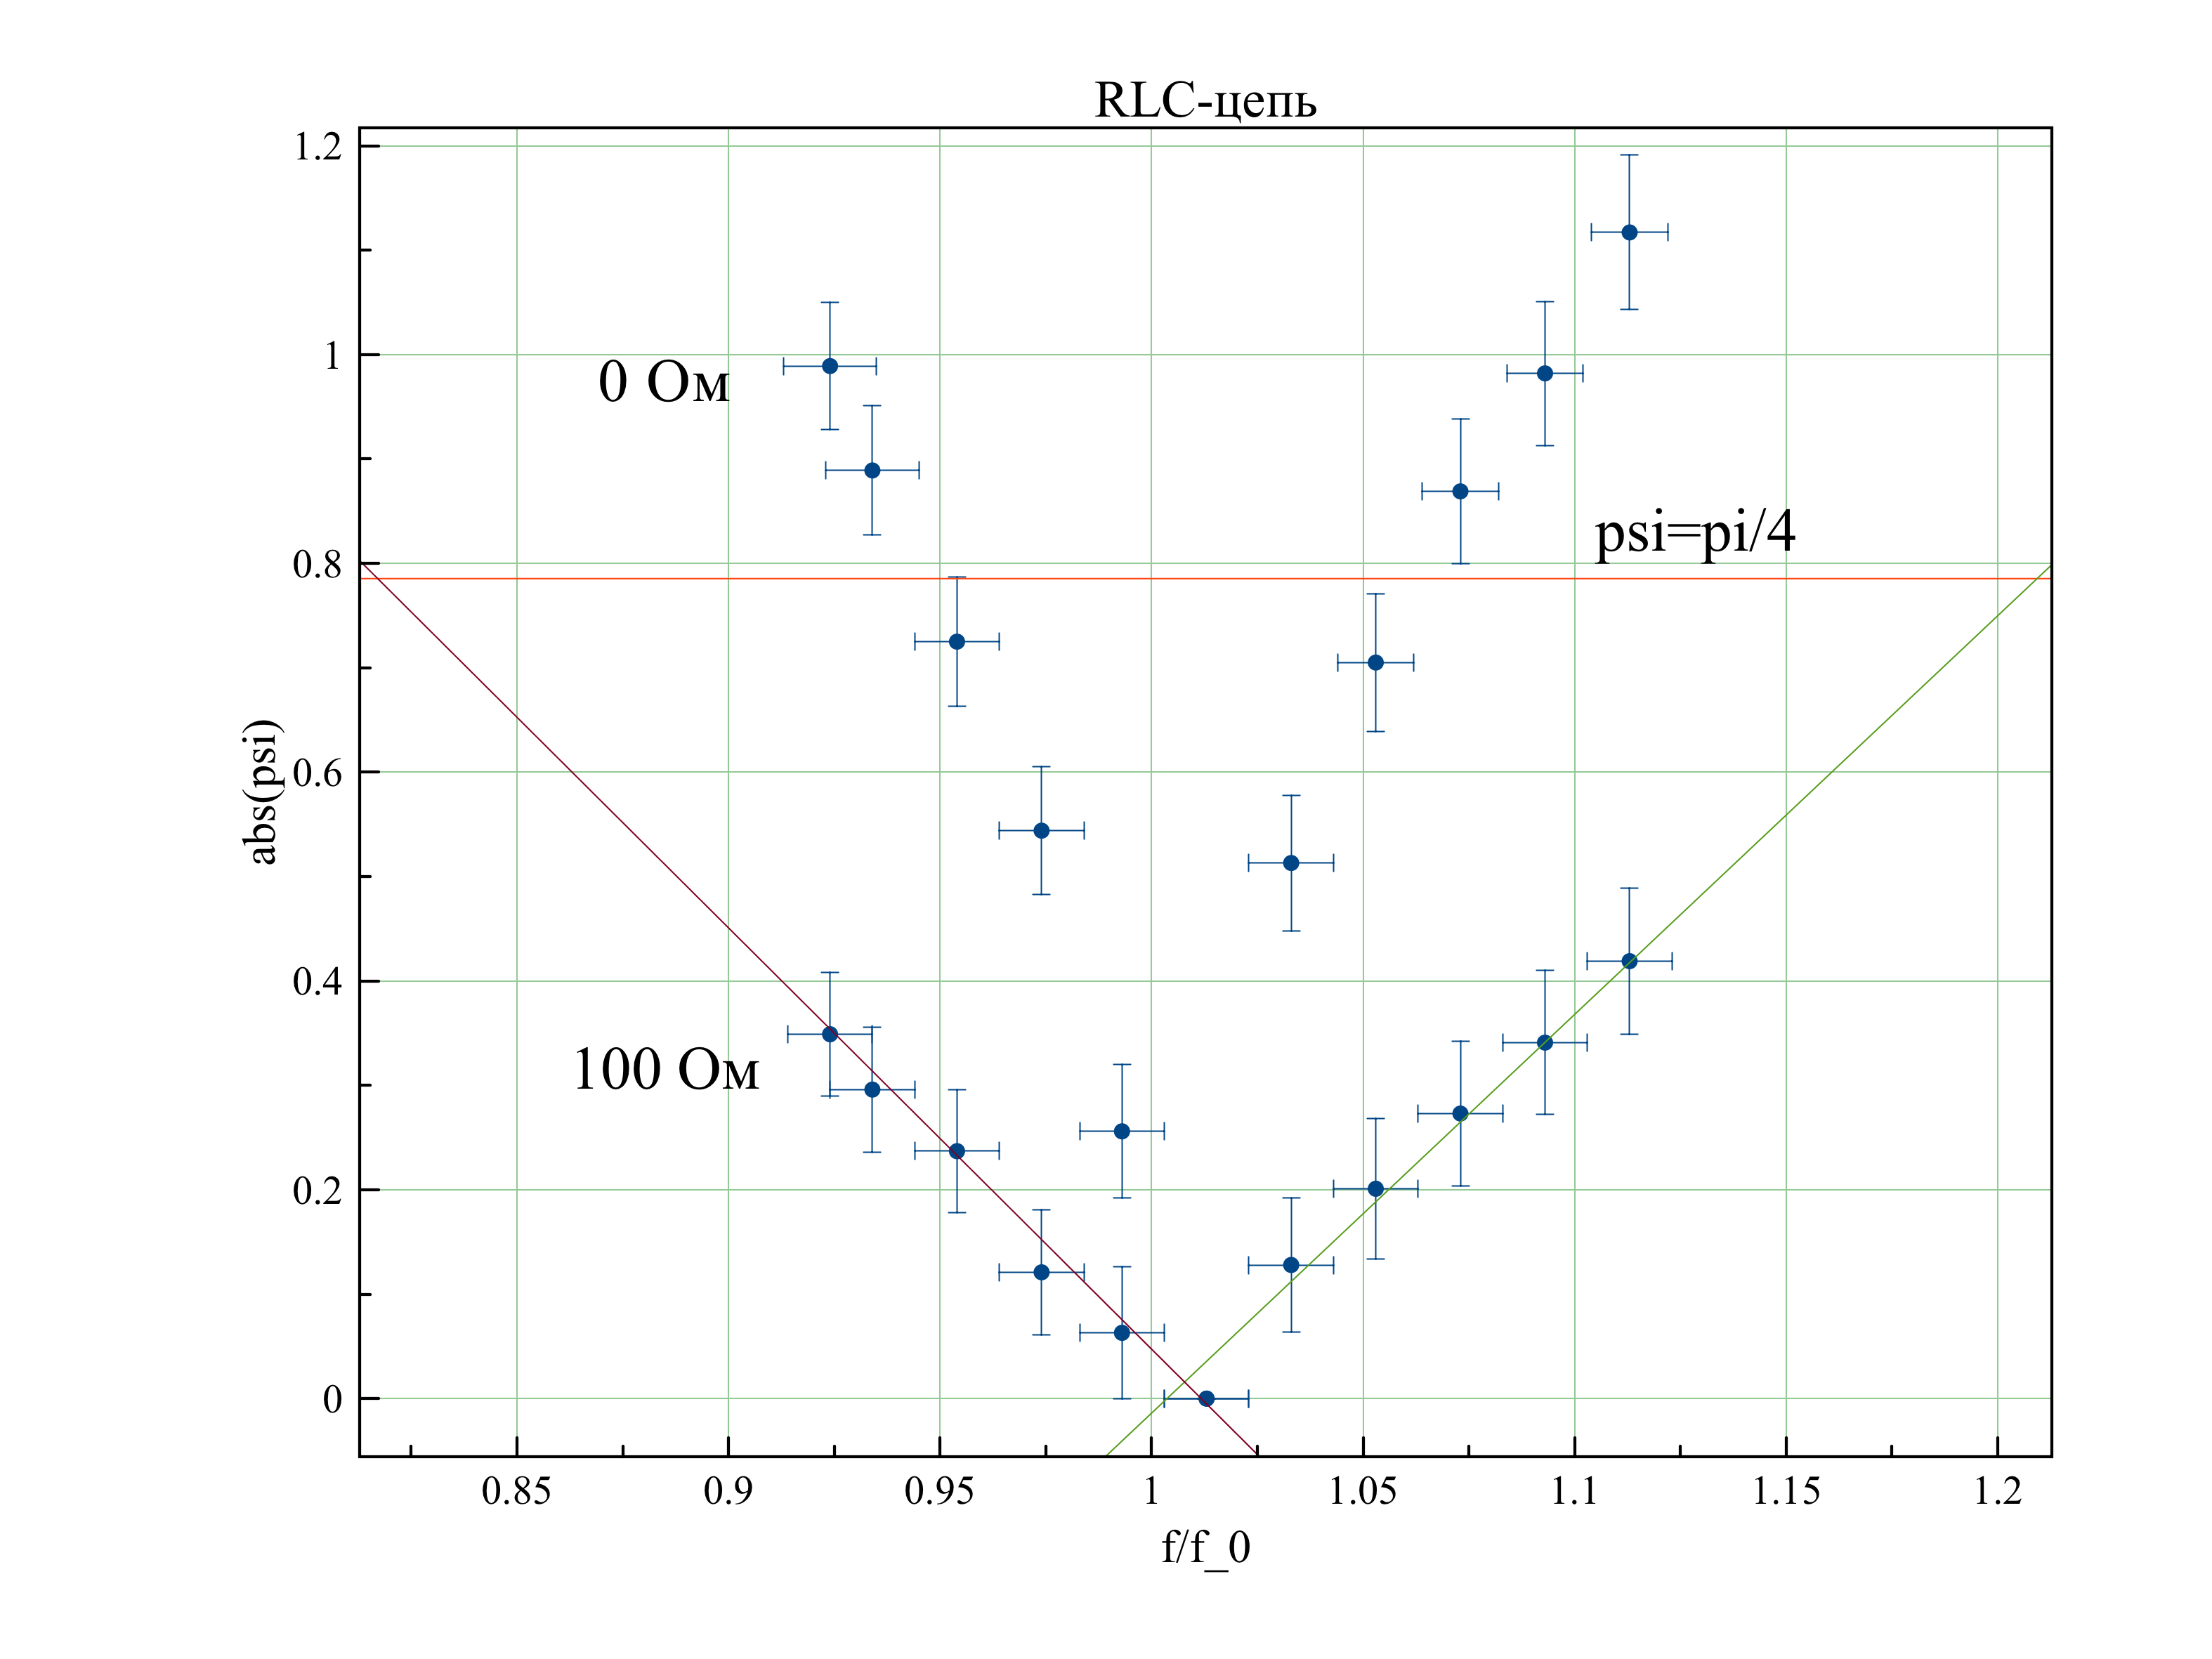
\includegraphics[width=0.8\textwidth]{RLC_help}
		\caption{Вспомогательный график для RCL-цепи для определения добротности}
	\end{center}
\end {figure}
Определим по графику добротность контура: $Q = \nu_0/(2\Delta\nu)$, где $2\Delta\nu/\nu_0$ -- ширина графика при сдвиге фаз $\psi = \pi/4$. \\

Из графика $R = 0$ Ом добротность равна:
$Q_{0}= 1/(1.07-0.94) = 7.7 \pm 0.6$

Из графика $R = 100$ Ом добротность равна:
$Q_{100}=2.5 \pm1.0$

Можно рассчитать её, выразив через параметры цепочки:
$$Q = \frac{1}{R} \sqrt{\frac{L}{C}}$$
$$Q_{\text{теор, 0}} = 7.2;~Q_{\text{теор, 100}} = 2.2$$

\section{Вывод}

В данной лабораторной работе была изучена зависимость сдвига фаз между током и напряжением от сопротивления в RC- и RL-цепи. Была определена добротность колебательного контура, снята зависимость сдвига фаз от частоты вблизи резонанса. 

Для RC и RL контуров практический график довольно точно совпадает с теоретическим в пределах погрешностей, что подтверждает теоретические рассуждения. При измерении добротности колебательного контура при $R=0$ Ом получились значения, практически совпадающие с теоретическими расчетами (с учетом погрешности). При измерении добротности в случае $R=100$ Ом получили достаточно большую погрешность, вследствии того, что напрямую точки не доходили до прямой $\pi/4$ -- построили предположительное продолжение кривой (см. рис.4). Но в итоге само значение добротности практически совпало с расчитанным теоретически.

\end{document}